\documentclass[5p,times]{elsarticle}

\usepackage{lipsum}

%% For including figures, graphicx.sty has been loaded in
%% elsarticle.cls. If you prefer to use the old commands
%% please give \usepackage{epsfig}

%% The amssymb package provides various useful mathematical symbols
\usepackage{amssymb}
%% The amsthm package provides extended theorem environments
%% \usepackage{amsthm}

% Please add the following required packages to your document preamble for tables:
\usepackage{booktabs}
\usepackage{graphicx}

%% Caption package for caption in figures and tables
\usepackage{caption}

%\journal{Nuclear Physics B}

%% Remove the line "Preprint submitted to Elsevier"
\makeatletter
\def\ps@pprintTitle{%
	\let\@oddhead\@empty
	\let\@evenhead\@empty
	\let\@oddfoot\@empty
	\let\@evenfoot\@oddfoot
}

\makeatother

\begin{document}


\begin{frontmatter}

\title{Predicting Effectiveness of a Mixed Integer Programming Model for the Concrete Delivery Problem\tnoteref{t1}}
\tnotetext[t1]{This document is the result of the final project
	of Applied Probability Models.}

\author{Oscar Alejandro Hernández López}
\address{Graduate Program in Systems Engineering, Universidad Autónoma de Nuevo León}
\ead{oscar.hernandezlpz@uanl.com.mx}

\begin{abstract}
The Concrete Delivery Problem (CDP) consists of the delivery of this product to different construction sites, named customers. In this project, the results of a solution method are analyzed to predict the chance to obtain an optimal solution, conditional on observable characteristics of the instances of this optimization problem.
As this variable is categorical it is used the nonparametric statistical Chi-Squared test in experimental work, as well as linear regression models that help to predict the probability of an instance of reaching an optimal value. Computational experiments with the results of the statistical methods are given that allow quantifying effects. 
\end{abstract}

\begin{keyword}
	Concrete Delivery Problem \sep Chi-Squared \sep hypothesis testing \sep linear probability model \sep categorical data
	%% keywords here, in the form: keyword \sep keyword
	
	%% PACS codes here, in the form: \PACS code \sep code
	
	%% MSC codes here, in the form: \MSC code \sep code
	%% or \MSC[2008] code \sep code (2000 is the default)
	
\end{keyword}

\end{frontmatter}

\section{Introduction}
	The CDP is a complex problem in logistics and optimization due to the nature of this product, which only can remain in concrete mixers for some time before it loses quality and hardens. Another factor is a maximum time lag constraint indicating a maximum time limit for two consecutive operations; this to assure the concrete's proper bonding between consecutive deliveries to the same customer. Also, clients demand a certain amount of product, which must be satisfied, and all of them have a specific time threshold to receive the material. As concrete distributors have a finite capacity, some clients can not be serviced during the operation. The objective is to maximize the number of satisfied customers according to their demand. 
	
	This work is motivated by the previous work conducted by \citet{hernandez2020study}, headed to propose efficient solution methods to tackle the CDP. With this research is an objective to estimate or predict the probability of an instance of the problem to reach an optimal value.
	
	This work is structured as followed. First, Section \ref{Section2} provides the main concepts associated with the problem and the used methods. Next, in Section \ref{Section3}, an overview of related research is presented. Section \ref{Section4} describes the proposed solution and the way is applied the Chi-Squared test as well as a linear probability model to the results of the solution method of the CDP. Section \ref{Section5} is devoted to show computational results. Finally, Section \ref{Section6} offers the conclusion.
	
\section{Background}\label{Section2}
	
	\citet{kinable2014concrete} proposed a variant of the CDP that contains most-real world constraints and provides instances available online that can be used to evaluate the performance of solution methods. Those instances are used in \citet{hernandez2020study}, where throughout proposing a compact Mixed Integer Programming (MIP) model the problem is solved, and data based on the obtained results are utilized to develop this work. Table \ref{tab:summary_instances} sums up all the characteristics of these instances. In the results, several variables are involved that characterize the performance of the solution method and this work is aimed at the analysis of those variables applying the study of statistics and probability models.
	 
	 \begin{table}[]
	 	\caption{Summary of Instances of the Concrete Delivery Problem}
	 	\label{tab:summary_instances}
	 	\begin{tabular}{@{}lll@{}}
	 		\toprule
	 		& \textbf{Dataset A}       & \textbf{Dataset B}       \\ \midrule
	 		\textbf{Instances}  & 64                       & 128                      \\
	 		&                          &                          \\
	 		\textbf{Customers}  & 10-20                    & 20-50                    \\
	 		Demands             & 10-75                    & 10-75                    \\
	 		Time Windows        & $ q_{i} \times {[1.1,2.1{]}}  $& $ q_{i} \times {[1.1,2.1{]}} $ \\
	 		Maximum Time Lag    & 5                        & 5                        \\
	 		&                          &                          \\
	 		\textbf{Vehicles}   & 2-5                      & 6-20                     \\
	 		Capacity            & 10-25                    & 10-25                    \\
	 		Classes             & 2-3                      & 3                        \\
	 		Processing time     & $ p_{k}=q_{k} $        & $ p_{k}=q_{k} $        \\
	 		&                          &                          \\
	 		\textbf{Stations}   & 1-4                      & 1-4                      \\
	 		Dist. Cust-Station  & 1-30                     & 1-30                     \\
	 		Dist. Depot-Station & 1-25                     & 1-25                     \\ \bottomrule
	 	\end{tabular}
	 \end{table}
	 
	 Random Variables represent features of systems and can be classified into two datatypes: numerical and categorical. The statistical data considered as categorical consists of variables that can take one of the limited possible values and are fundamental for this research.
	 
	 Simulation is essential as well since it allows to analyze the alternatives to optimize systems, recognize the impact of modifications or, where appropriate, the irrelevance of the actions, and predict its behavior.
	 
	 Prediction modeling has been widely used in statistical practice and a typical approach is to determine the statistical significance of an observed association between an indicator and the outcome, controlled by variables denoted as predictors. This may conduct hypothesis testing, as an example of statistic inference. This involves formulating a statistical hypothesis using sample data to decide on the validity of the formulated statistical hypothesis and is the basis of this work.
	 

\section{Related Work}\label{Section3}
	
	According to \citet{ilakovac2009statistical}, there is a procedure to do any hypothesis testing, although details might change from one test to another. It begins by setting up the null and alternative hypotheses. Then one can define the test procedure, including the selection of significance level. Besides, calculate test statistics and associated $p$-value and finally conclude that data are consistent or inconsistent with the null hypothesis. It is important to have in mind that associated with this decision two possible errors are present. The first is the Type I error and occurs when the effect is seen when actually there is none and the probability of making this type of error is usually called alpha ($\alpha$). On the other hand, Type II error occurs when one fails to discern any difference when it is actually present. By convention $p$-value greater than 5\% is called ``not significant" and sometimes the term wrongly implies that the study has shown that there is no difference, whereas usually what shows is an absence of evidence of a difference \cite{altman1995statistics}. 
	
	\citet{napierala2012bonferroni} mentions that to reduce the chances of obtaining type I errors (false-positive) results the Bonferroni correction is used when multiple pairwise tests are performed on a single dataset. Then, this is an adjustment made to $p$-values when several dependent or independent statistical tests are being performed simultaneously.
	
	Many statistical methods require assumptions, depending on the format of the data to be analyzed, and are situations in which even transformed data may not satisfy these assumptions, and in those cases, it may be inappropriate to use parametric methods of analysis. Nonparametric methods provide an alternative series of statistical methods that require no or very limited assumptions to be made about the data \cite{whitley2002statistics}.
	 
	The Chi-Squared ($\chi^{2}$) test is a nonparametric statistical test that determines if two or more samples are independent or not. \citet{zibran2007chi} states that for the purpose of the test, as it can only be applied to discrete data, continuous data can be often put into a discrete form by the use of intervals on a continuous scale. \citet{camilli1978applicability} prove that the $\chi^{2}$ test for 2 $\times$ 2 contingency tables give accurate probability statements of Type I error. Besides, once the $\chi^{2}$ is stated to be significant, \citet{shan2017fisher} explain the next step is performing a post hoc test to find out the cells from the respective contingency table that differs from their expected values and the larger these residuals are, the greater the contribution to the overall chi-squared test.
	
	Chi-Squared tests are used for testing hypothesis about one or two categorical variables. It is appropriate when data can be summarized by counts or frequencies in a table, usually contingency tables. For one categorical variable the $\chi^{2}$ goodness of fit test can be performed. It begins with the hypothesis that the distribution of a variable behaves in a particular manner. In the case of two categorical variables one can perform a $\chi^{2}$ test for association, to test the null hypothesis that the variables are independent  \cite{charles1997introduction}.
	
	As nonparametric methods are suited toward hypothesis testing rather than estimation of effects \cite{whitley2002statistics}, in case of effect or differences between groups are statistically perceived, an alternative might be interested in extent comparisons of effects by estimating and interpreting them either by linear models and when facing discrete outcomes by the probability, logit or probit model \cite{holm2015comparing}.
	
	A linear regression model \cite{myers1990classical}, with a dependent variable that is either zero or one is called the linear probability model \cite{aldrich1984linear}. According to \cite{cleary1982estimation} in linear models with only first-order terms, all independent variables are assumed to have main effects (an effect of a risk factor that is constant, irrespective of the presence or absence of other factors). The first-order term in this sort of model is referred to as a conditional effect and is the effect of a factor at a particular value of other modified influences.
	
\section{Methods}\label{Section4}

	Data collected corresponds to the results of \citet{hernandez2020study}. In this mentioned work a Compact MIP model is proposed in order to tackle the CDP. Benchmark data used are available at  \cite{kinable2013dataset}.
	As initial step variables of interest are analyzed as part of an exploratory data analysis.
	The possible outcomes for a solution can be Optimal or Non Optimal, for the different datasets (A or B), and is the dependent variable. As it has categorical values a $ \chi^{2}$ test is performed to check if there is a relationship between those variables. 
	
	Chi-Squared test involves calculating a number called the chi-square statistic - $\chi^{2}$. The formula for the $\chi^{2}$ statistic is: \begin{equation}
		\chi_{c}^{2} =\sum_{i=0}^{n} \frac{\left( \mathbb{O}_{i} - \mathbb{E}_{i}\right) ^{2}}{\mathbb{E}_{i}}, 
	\end{equation} where the subscript $ \textit{c} $ referes to the degrees of freedom, $\mathbb{O}$ is the observed value and $\mathbb{E} $ is the expected value. This sumation indicates one have to perform a calculation for every single data item in the dataset.
	
	The number of degrees of freedom $ n $ of the random variable $\chi^{2}$ is the parameter of the chi-squared density, and it is determined by the expression $ (a-1)(b-1) $, where $a$ and $b$ are, for example, values of two traits being checked for independence. The null hypothesis for the $\chi^{2}$ test are of independence is that two categorical variables are independent in some population. Usually, it can be said two variables are related when the null hypothesis of independence is rejected if $p$-value<0.05.
	
	After performing a Chi-Squared Test, in case of relation, it is appropriate to describe this effect, in order to explain the behavior of the dependent variable throughout a linear probability model. 
	
	The linear regression model has the form: \begin{equation}
		Y_{i} = \beta_{0} + \beta_{1}X_{1i} + \beta_{2}X_{2i} + ... + \beta_{k}X_{ki} + u_{i}.
	\end{equation} This model with a binary dependent variable $Y_{i}$ is called a linear probability model \cite{hanck2019introduction}, and \begin{equation}
		P(Y_{i} = 1 \mid X_{1},X_{2},...,X_{k} ) = \beta_{0} + \beta_{1} + X_{1i} + \beta_{2}X_{2i} + ... + \beta_{k}X_{ki},
	\end{equation} therefore, $ \beta_{j} $ is interpreted as the change in the probability that $ Y_{i} = 1 $, holding constant the other $ k -1$ regressors.
	
	All the steps of this described methodology are performed using R software in its version 4.0.2 \citep{r}, and run on a MacBook Air with an Intel Core i5 CPU $ @ $ 1.8 GHz and 8 GB RAM. The code used is available on the GitHub repository \citep{github}.


\section{Results} \label{Section5}
	
	  Instances are classified in two datasets (see Figure \ref{fig:pie1}). Dataset A contains instances with 10-20 customers and 2-5 vehicles, being the smaller ones. On the other hand, Dataset B has up to 50 customers and 20 vehicles.  Instances are generated as follows: demands of customers are always divisible by 5 and are selected at random from the interval $  \left[ 10-75\right] $, as well as the capacities of the $ k $ vehicles, are selected between $ \left[ 10-25\right] $. The processing time of a vehicle is proportional to its capacity. The width of the time window of a customer $i$ is computed by $ \lambda_{i}q_{i} $, where $ \lambda_{i} $ is a scalar uniformly selected from the interval $\left[1.1-2.1\right]  $. Locations lay in the euclidean plane, travel time between two locations equals the euclidean distance, rounded upwards. Distance between each station and depots is uniformly selected from the interval $ \left[ 1-30\right ]$, and for each customer, there exists a plant within a distance of $ \left[ 1-25\right]   $. The time lag is fixed to 5 for all deliveries. 
	  
	\subsection{Data Exploration}
			
		The exploration process starts with the analysis of relevant variables in order to better understand their distributions by convenient representations. Figure \ref{fig:pie1} shows the number of instances of the CDP, where the 67\% of them belongs to group B (larger instances). Figure \ref{fig:barplot} shows a counting of the categorical variable that represents if an instance has reached an optimal value or not. Instances with 5-20 customers present a higher percent of reaching optimal values, whereas the proposed solution method shows minor effectiveness. This effectiveness can be outlined by the analysis of the Gap, which is a measure of proximity between the reached value in the objective function (Bound) and the optimal solution. Figure \ref{fig:boxplot} is a representation of this measure and shows the respective Gaps of the solutions, grouped by customers. The distribution of these objective values reached by instances is represented in Figure \ref{fig:histogram}.
			
			\begin{figure}
				\begin{center}
					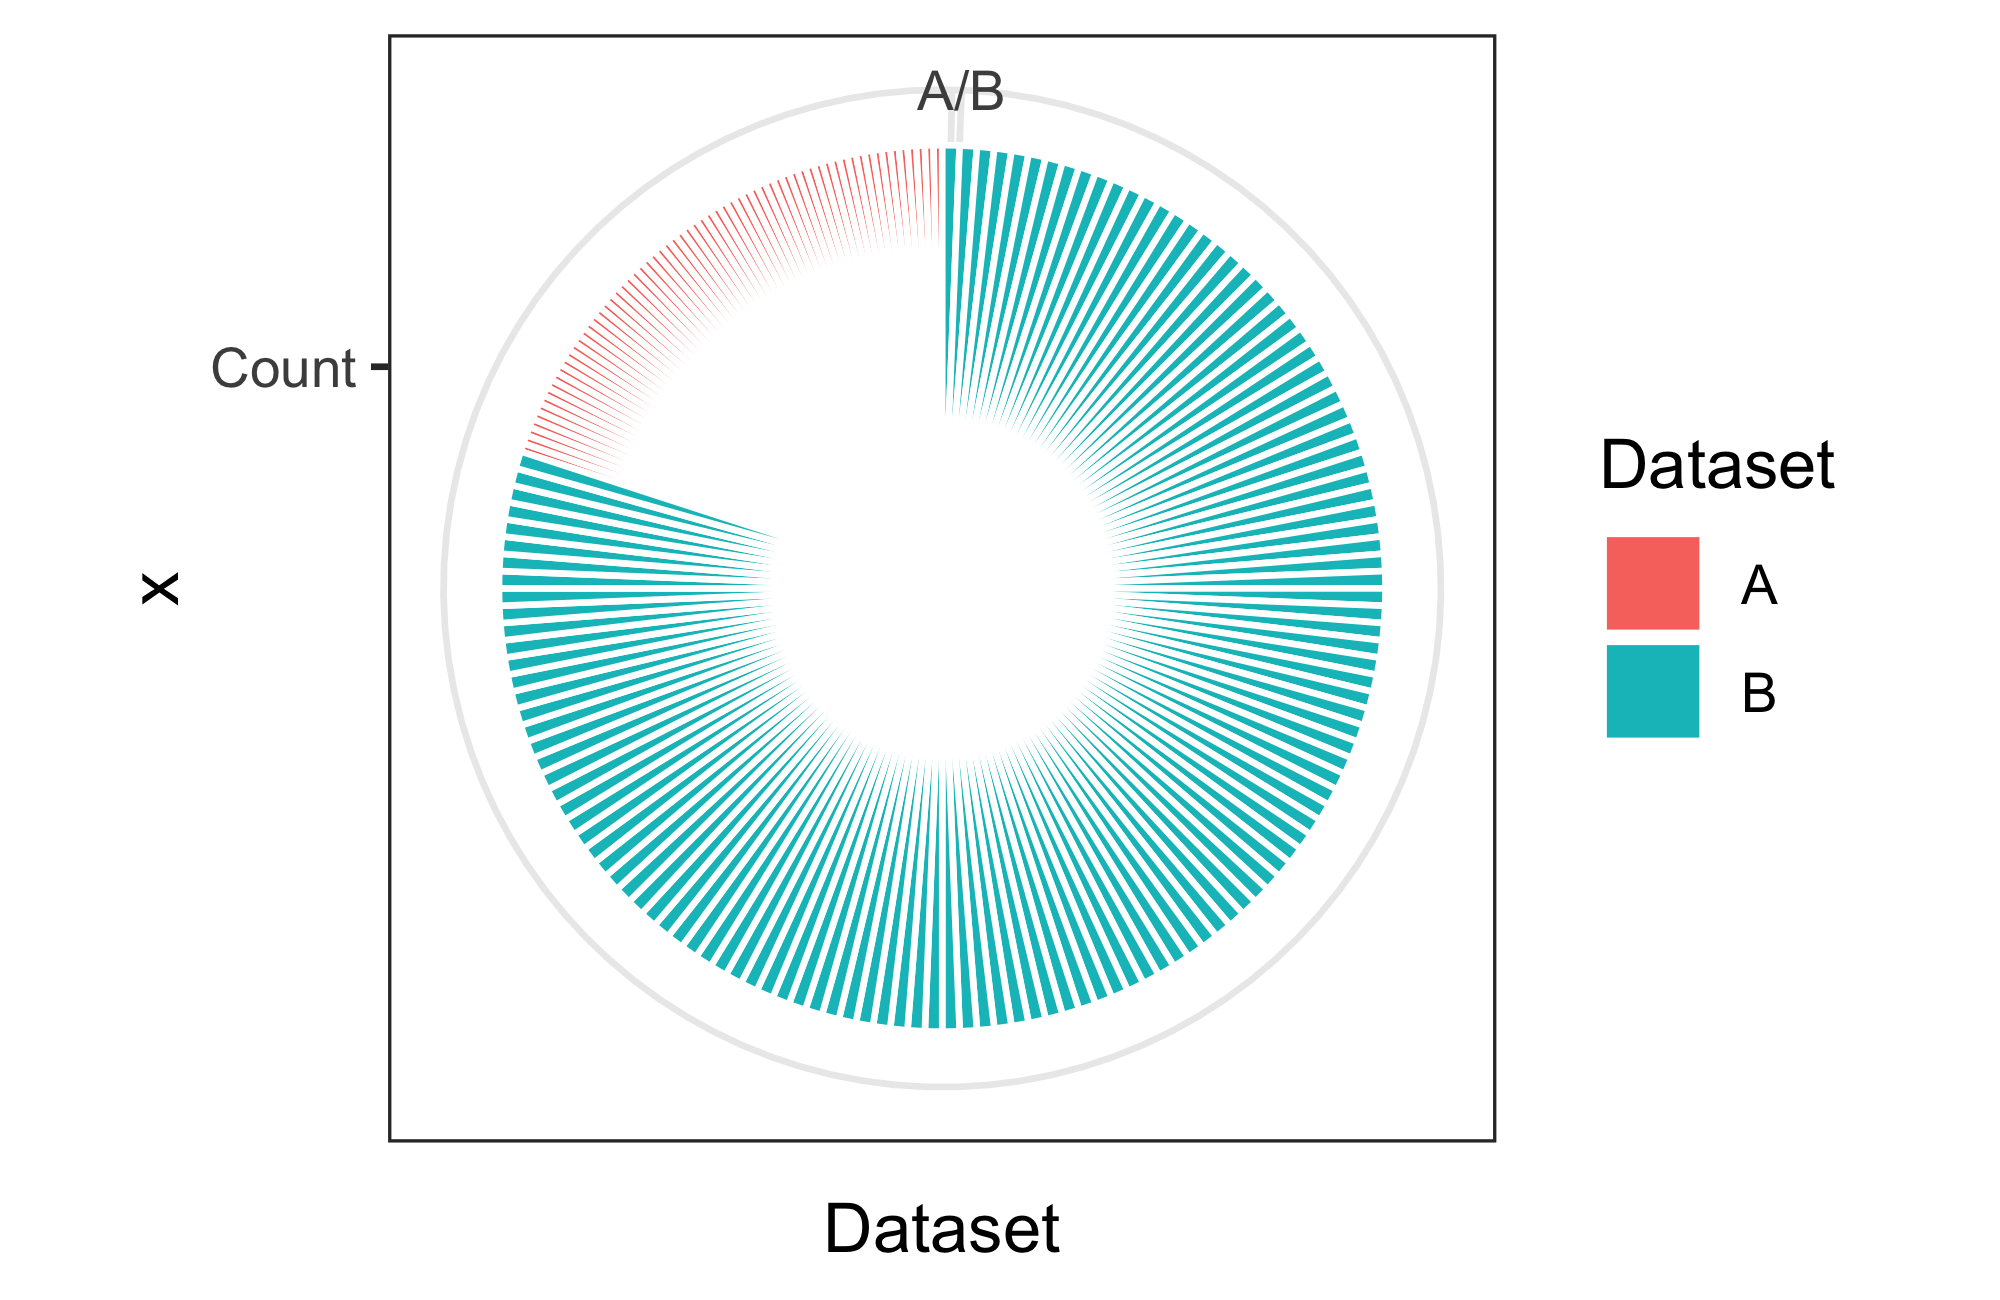
\includegraphics[scale=0.11]{fig/pie_dataset}
					\captionof{figure}{Group of Instances by Dataset }
					\label{fig:pie1}
				\end{center}
			\end{figure}

			\begin{figure}
				\begin{center}
					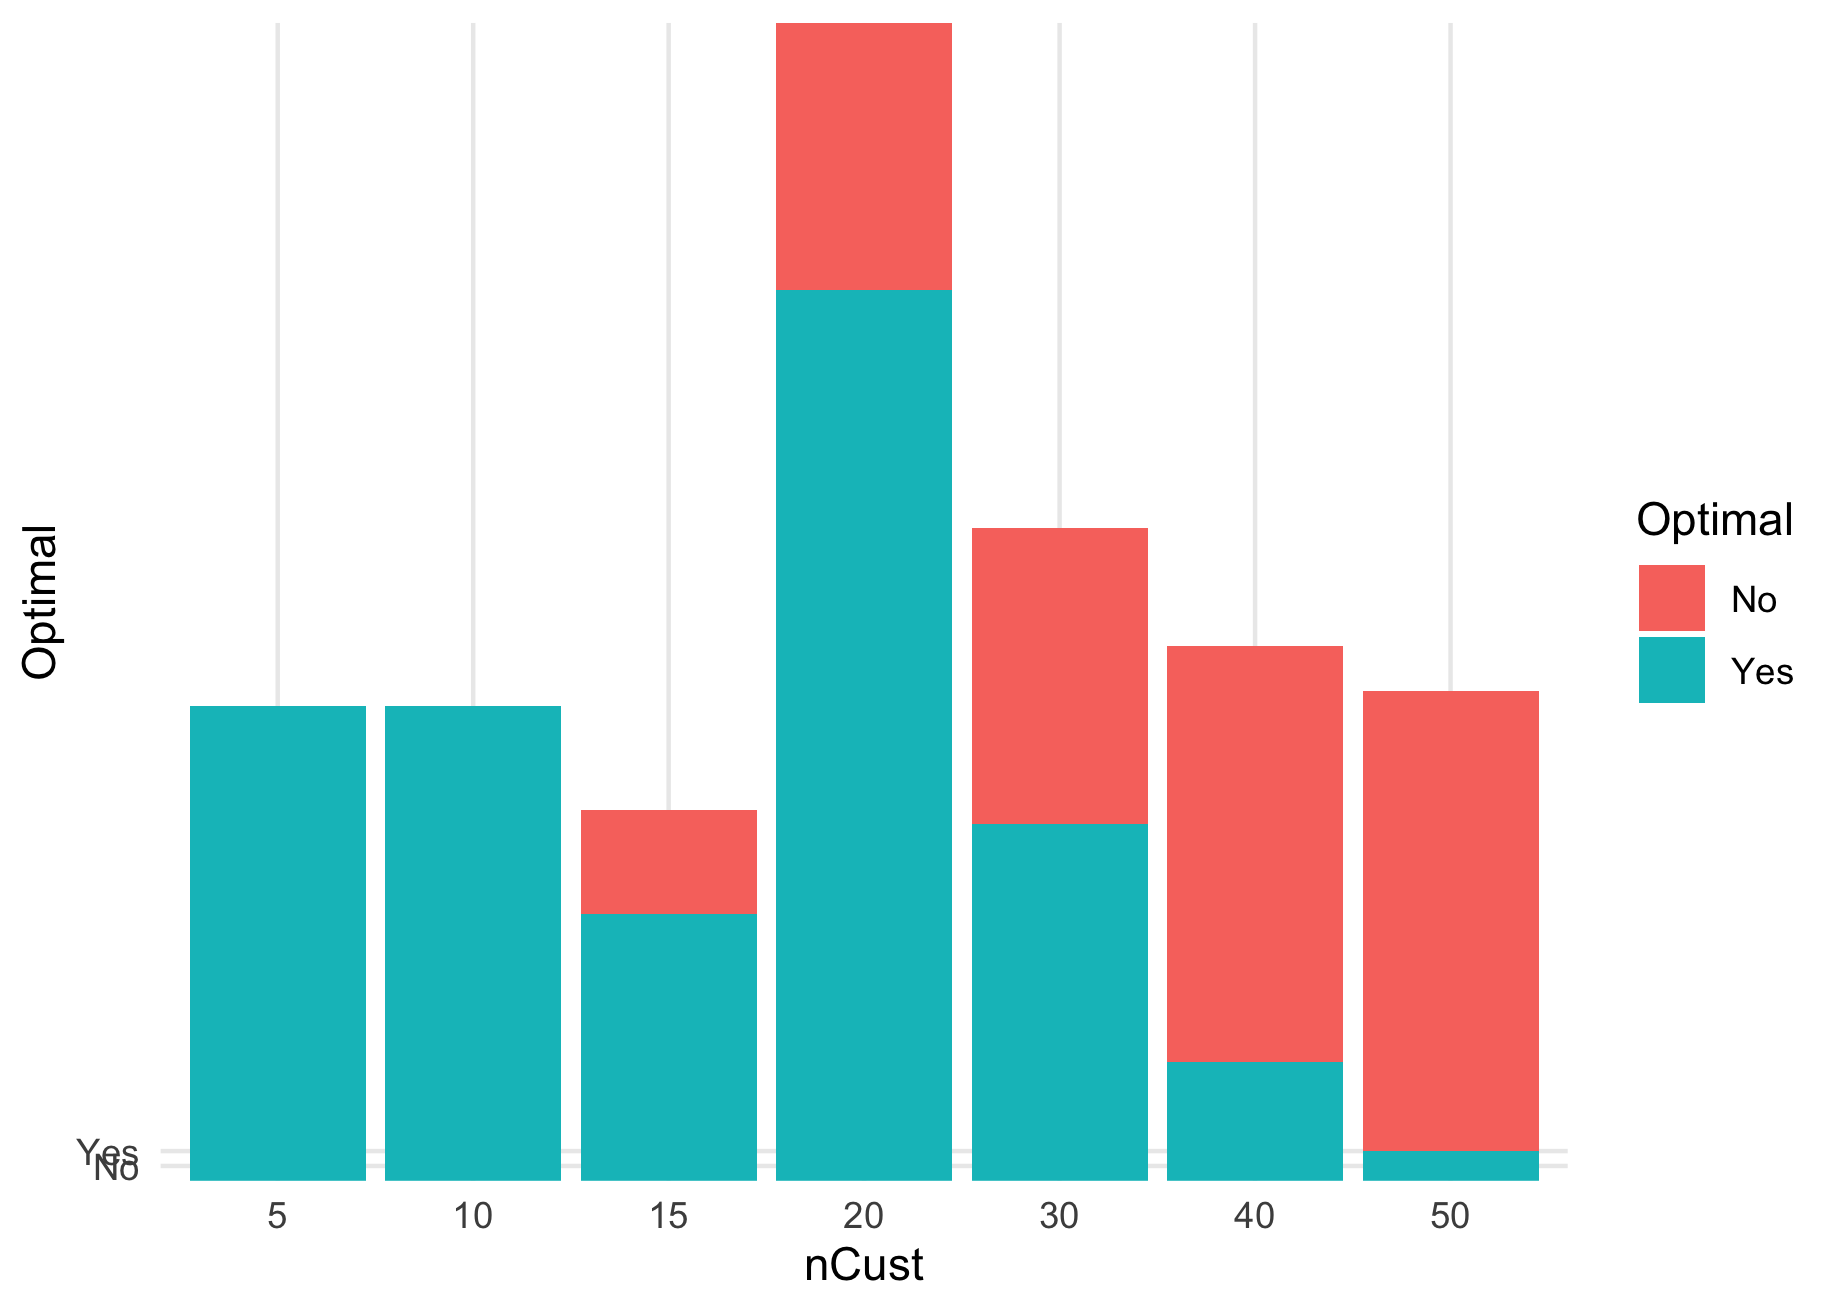
\includegraphics[scale=0.11]{fig/barplot}
					\captionof{figure}{Barplot of \textit{Optimal Values} by group of customers}
					\label{fig:barplot}
				\end{center}
			\end{figure}
	
			\begin{figure}
				\begin{center}
					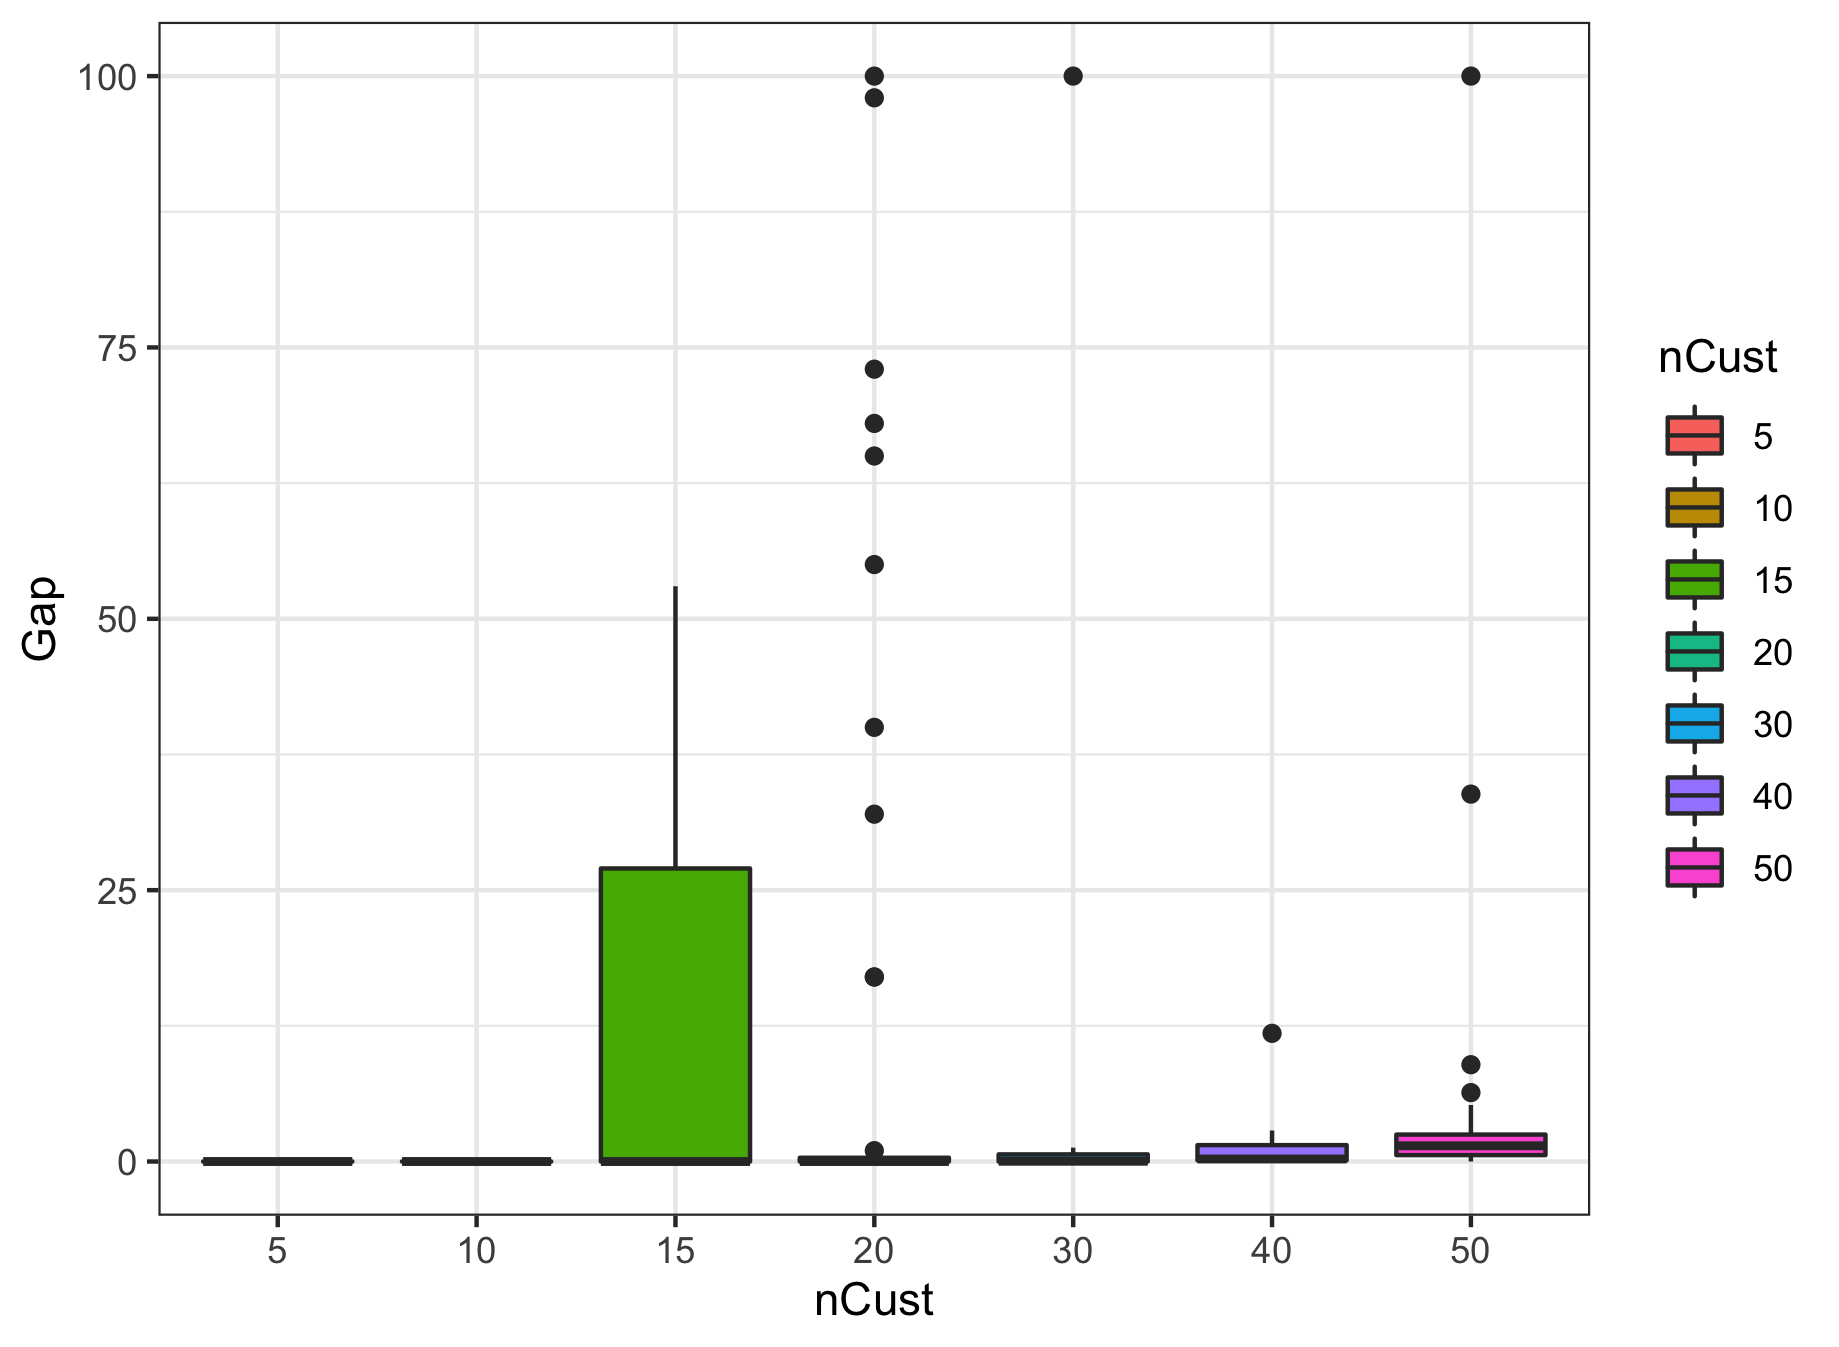
\includegraphics[scale=0.11]{fig/boxplot}
					\captionof{figure}{Boxplot of the Gap of solutions by group of customers}
					\label{fig:boxplot}
				\end{center}
			\end{figure}

			\begin{figure}
				\begin{center}
					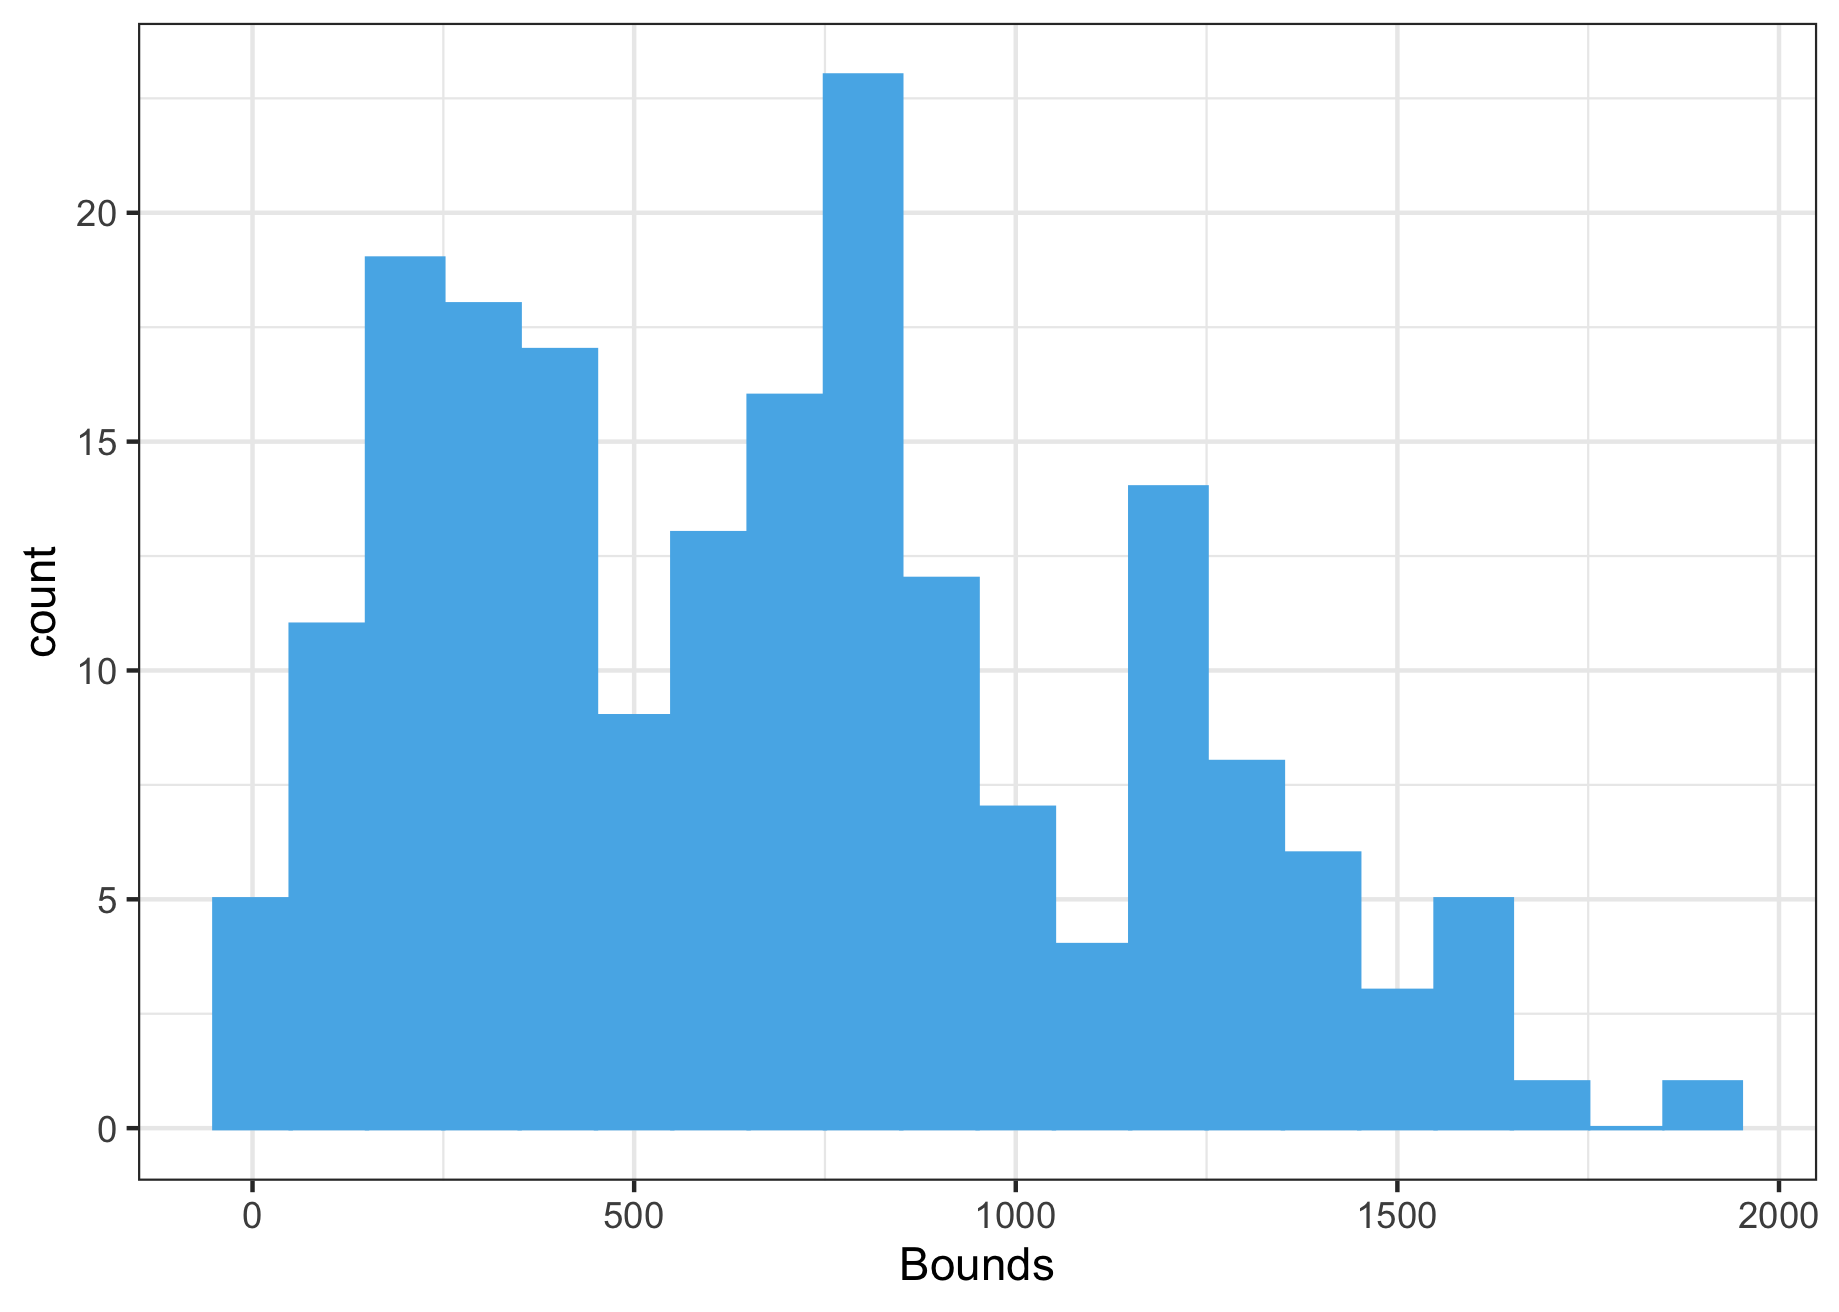
\includegraphics[scale=0.11]{fig/histogram}
					\captionof{figure}{Histogram of the variable \textit{Bounds} obtained by Instances }
					\label{fig:histogram}
				\end{center}
			\end{figure}
	
	\subsection{Chi-Squared Test}
	
		Chi-Squared test of independence is conducted to evaluate if a relationship between the variables in the population. For variables \textit{Dataset} and \textit{Optimal} a $p$-value of $1.33 \times 10^{-7}$ is obtained, which is less than the significance level of 5\%; in this context means the null hypothesis that the variables are independent ($H_{0}$: there is no relationship between a Dataset and the Outcome of an Instance) can be rejected. As there is a significant relationship between the Dataset and the Outcome, knowing the value of one variable helps to predict the value of the other variable.
		
			\begin{figure}
				\begin{center}
					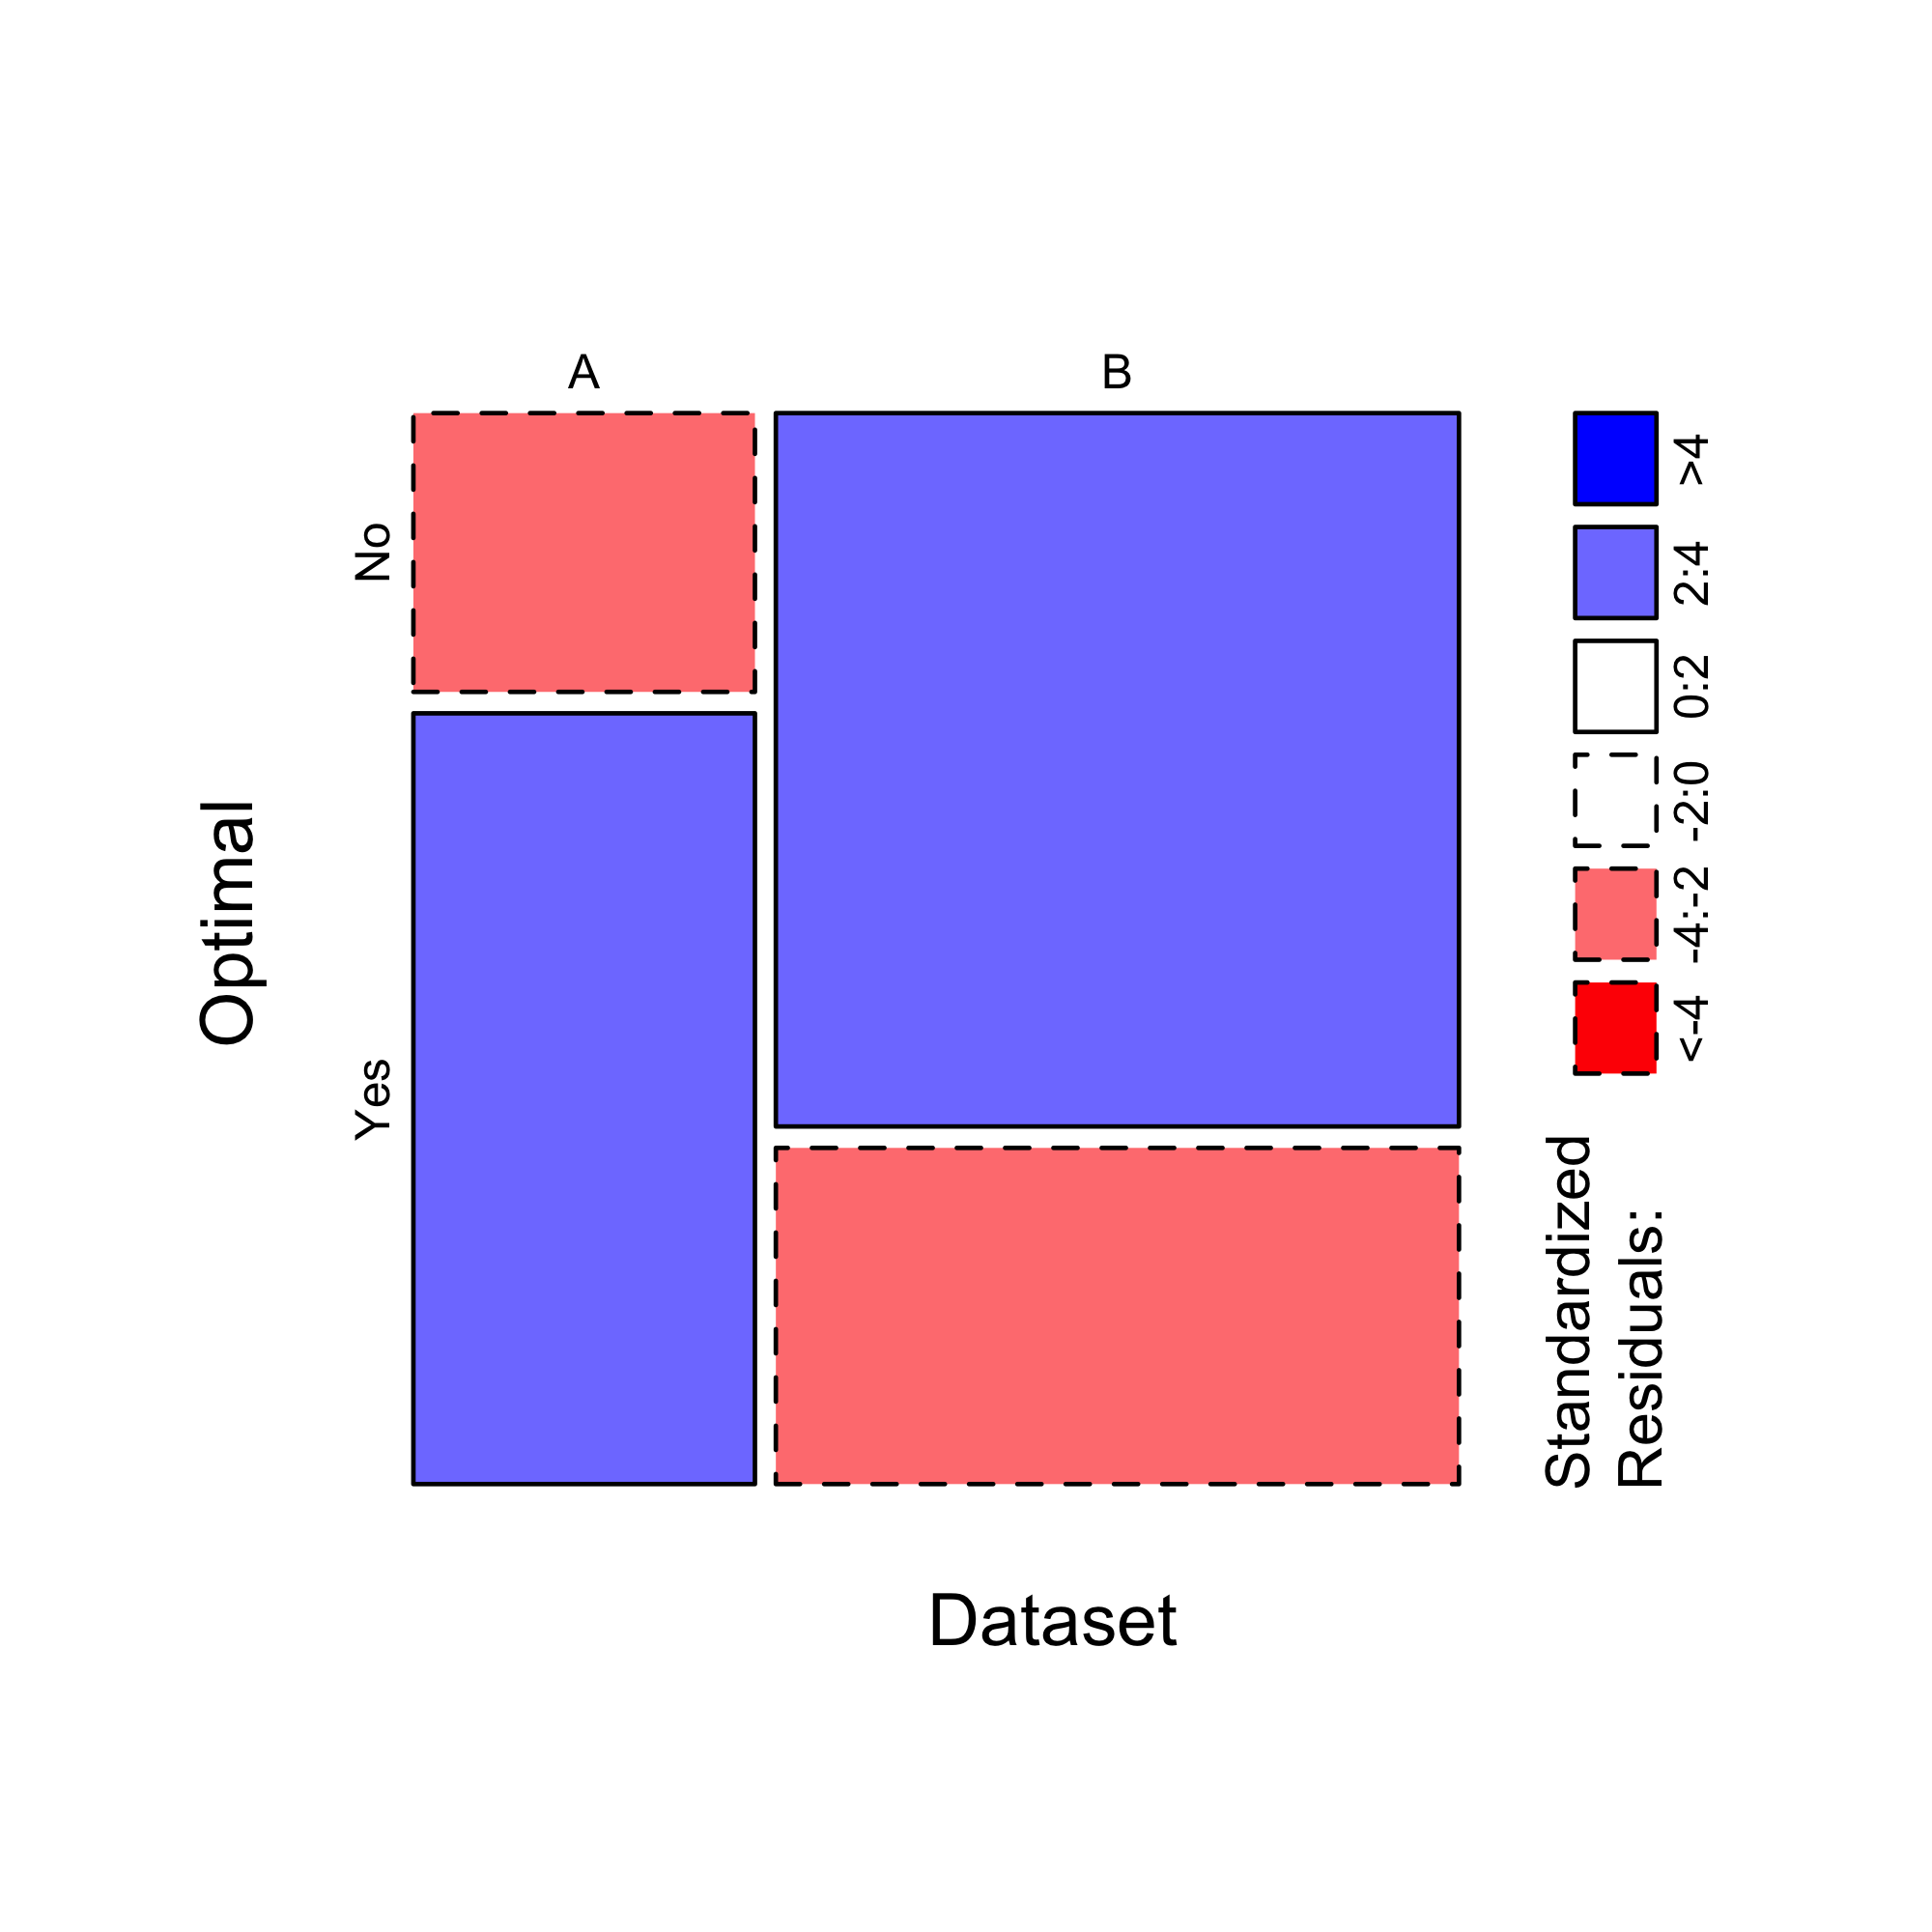
\includegraphics[scale=0.09]{fig/mosaicplot}
					\captionof{figure}{Mosaic plot for \textit{Optimal} vs \textit{Dataset} }
					\label{fig:mosaicplot}
				\end{center}
			\end{figure}
	
	\subsection{Post Hoc Testing}
	
		At this point, it has been proven statistically a significant relationship between the Dataset and if a solution turns out to be optimal or non-optimal (Outcome). Post hoc testing enables understanding of which categories are contributing to this significance and how. Classification in Datasets is given by the number of customers to be covered, that is why it is decided to stratify this variable by this number. Therefore this part of the analysis is given by a similar relation between the number of customers and the possible outcome. This test is performed using R software and its \texttt{chisq.posthoc.test} package. In this test adjusted standardized residuals are used accompanied by the $p$-values of each relation applying a Bonferroni correction. As a result, instances that show relationships with a $p$-value less than the corrected and turned out to be statistically significant are the instances with 5 and 10 customers, with $p$-values of $7.8 \times 10^{-5}$ and instances with 40 or 50 customers, with $p$-values of $4.74 \times 10^{-4}$ and $2 \times 10^{-6}$ respectively.
	
	\subsection{Linear Probability Models}
	
		The variable interested in modelling is \textit{Optimal}. A regressor that might have power in explaining whether an instance has reached an optimal value is \textit{nCust}, which is the number of customers to be served in a given instance. It can be translated into the simple regression model \begin{equation}
			Optimal = \beta_{0} + \beta_{1}\times nCust + u
		\end{equation} and is estimated using the \texttt{lm()} function of R software. As a result coefficients of -0.0221 for \textit{nCust} and 1.0660 as Intercept are obtained. Therefore, the estimated regression line is: \begin{equation}
			\widehat{Optimal} = 1.066 - 0.022 \times nCust.
		\end{equation} Figure \ref{fig:lm} shows this data as well as the regression line. The model indicates a negative relation between the number of customers to be served and the probability of obtaining an optimal solution so instances with higher clients are more likely to not reach the optimal. According to the model, an instance with 30 customers is associated with an expected probability of not reaching an optimal value of roughly 50\%.

			\begin{figure}
				\begin{center}
					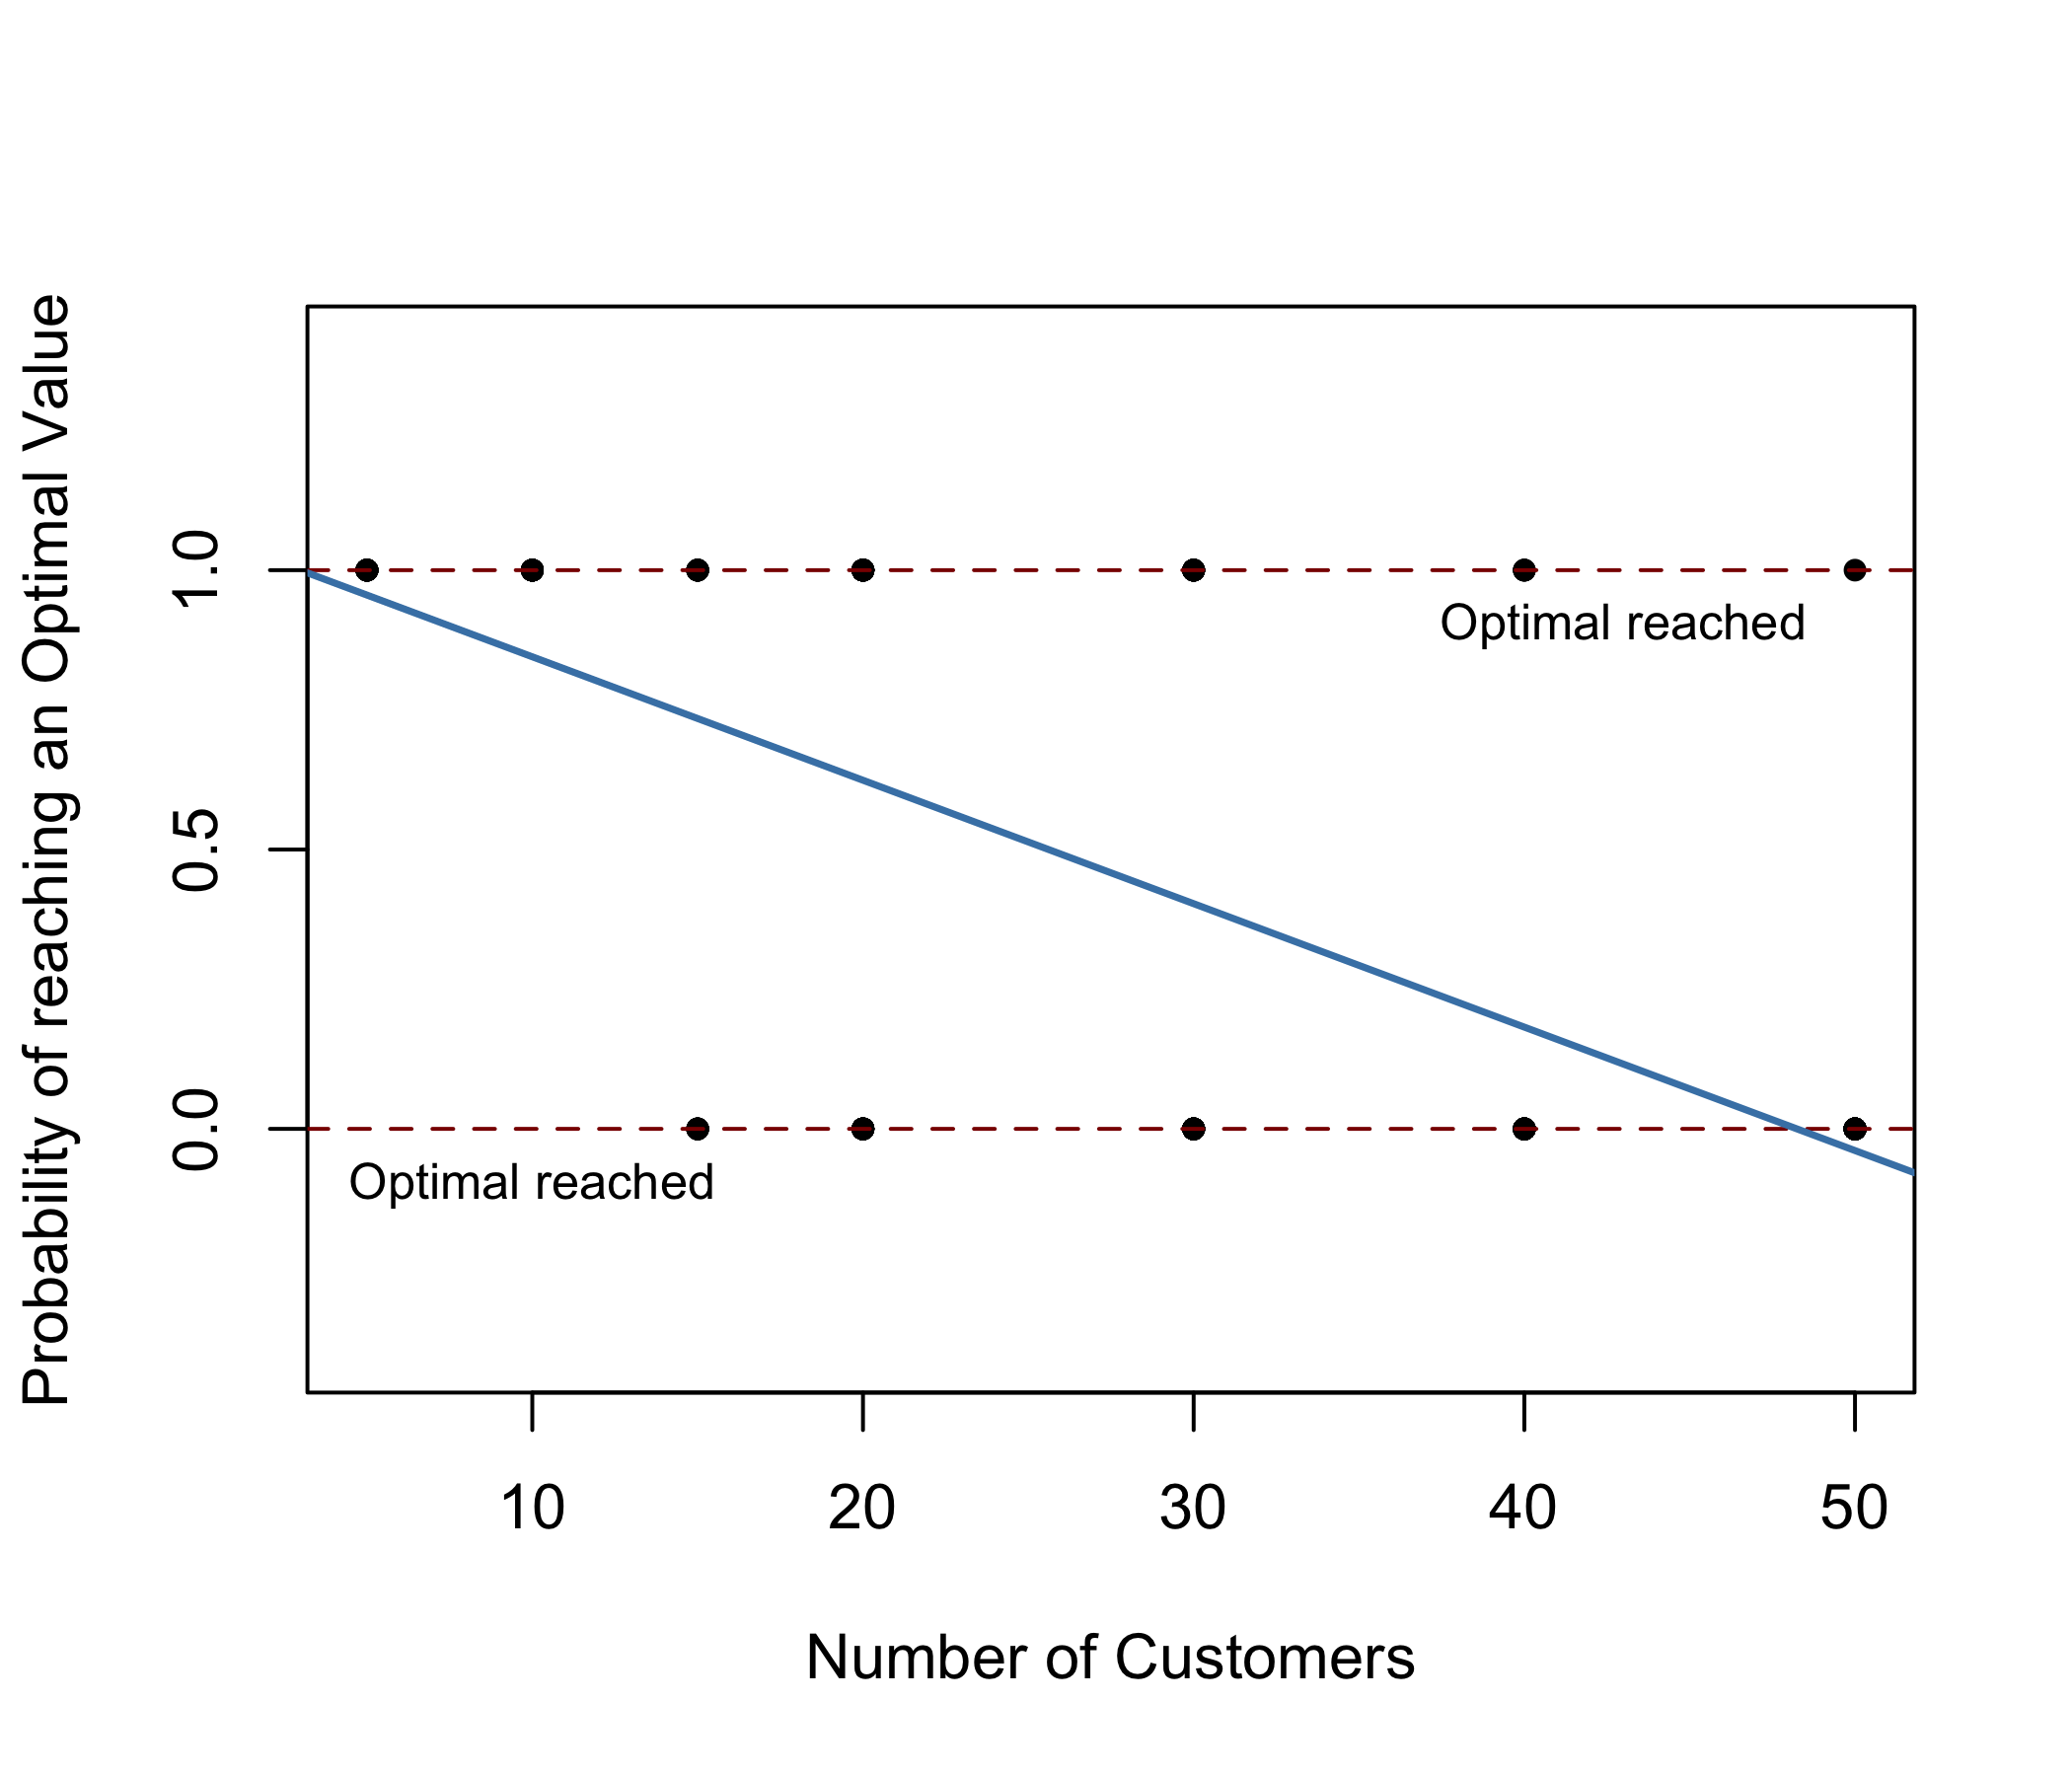
\includegraphics[scale=0.09]{fig/pred}
					\captionof{figure}{Scatterplot for Optimal Result vs Amount of Customers}
					\label{fig:lm}
				\end{center}
			\end{figure}
		
		Furthermore, additional regressors can be added as the \textit{CPU time}, and the \textit{nVehicles} (number of vehicles). This variable ought to be able to explain the status of a solution. It is set with a limit and is expected to reach it if the instance has not reached an optimal value, on the other hand, one can come up with the conjecture that the higher the time the program is running, the more chance it might reach an optimal. Such influence is modeled the same as the previous model, and as a result, both coefficients are -0.0015 (\textit{nCust} and \textit{CPU time}), whereas the Intercept is 0.9500. The estimated regression function is: \begin{equation}
			\widehat{Optimal} = 0.9500 - 0.0015 \times nCust. - 0.0015 \times CPU time.
		\end{equation} The coefficient on $ CPU time $ is negative, indicating that holding constant the number of customers, a higher value of the CPU time not necessary means a higher probability of reaching an optimal value.
 
\section{Conclusions} \label{Section6}
	
	Statistical methods are a very useful tool to understand the behavior of variables, that sometimes might be related somehow. Hypothesis tests are authentic examples that allow detecting if this relation exists being the basis to further explain the effect some variables may have on others. $\chi^{2}$ test can tell whether some sort of classifications on a given population are independent of each other or not. Then, Linear Regression Models can complement the results, if the situation requires and conditions are appropriate.
	
	In this work $\chi^{2}$ test of independence is applied to observe if there is a relationship between the result of a given instance (if is optimal or not) and other specific characteristics of it. Once the relation is evidenced, a linear probability model is obtained that allows to identify the grade of the importance of these characteristics in the result and predicts the probability of reaching an optimal value.
	
	As future work, since all instances with 5 and 10 customers have reached optimal values, experiments increasing randomly demands within a permitted rank are being performed to evaluate the impact of uncertainty of this parameter in the objective function, and have another measure of the robustness of the solution method. In addition, it is aimed to develop a heuristic procedure for solving this problem and tackle the larger instances that also have an influence on the results and then execute the proper experimentation to evaluate the performance.

%% If you have bibdatabase file and want bibtex to generate the
%% bibitems, please use
%%
\bibliographystyle{elsarticle-harv} 


%Offered Elsevier's bibliography styles that I could activate:
%% Numbered
%\bibliographystyle{model1-num-names}

%% Numbered without titles
%\bibliographystyle{model1a-num-names}

%% Harvard
%\bibliographystyle{model2-names}\biboptions{authoryear}

%% Vancouver numbered
%\usepackage{numcompress}\bibliographystyle{model3-num-names}

%% Vancouver name/year
%\usepackage{numcompress}\bibliographystyle{model4-names}\biboptions{authoryear}

%% APA style
%\bibliographystyle{model5-names}\biboptions{authoryear}

%% AMA style
%\usepackage{numcompress}
%\bibliographystyle{model6-num-names}

%% `Elsevier LaTeX' style
%\bibliographystyle{elsarticle-num}

\bibliography{ref}
\end{document}